\newpage
\chapter{Заряженная частица в однородном магнитном поле}
\par  Рассмотрим задачу о постоянном однородном электромагнитном поле. Нужно найти $\psi$ и $E$:
$$\frac{\left(\hat{\vec{p}} - \frac{e}{c} \vec{A}(\vec{r}) \right)^2}{2m}  \psi = E \psi$$
\par \textbf{1. Ищем векторный потенциал.} $\vec{B}= \mu \vec{H}$, $\vec{H} \uparrow \uparrow \vec{z}$.
\par
$$rot \vec{A} = \left |\begin{matrix} \vec{x}_0 & \vec{y}_0 &\vec{z}_0  \\ \frac{\partial}{\partial x} & \frac{\partial}{\partial y} &\frac{\partial}{\partial z} \\ A_x & A_y & A_z \end{matrix} \right| = \vec{x}_0 \left(\frac{\partial}{\partial y}A_z - \frac{\partial}{\partial z} A_y\right) -  \vec{y}_0 \left(\frac{\partial}{\partial x} A_z - \frac{\partial}{\partial z}A_x  \right) + \vec{z}_0 \left(\frac{\partial}{\partial x}A_y -  \frac{\partial}{\partial y}A_x   \right) $$
\par Т.к. $\vec{B}$ имеет только одну компоненту, то $$\frac{\partial}{\partial y}A_z - \frac{\partial}{\partial z} A_y = 0 \qquad \frac{\partial}{\partial x} A_z - \frac{\partial}{\partial z}A_x  = 0 \qquad \frac{\partial}{\partial x}A_y -  \frac{\partial}{\partial y}A_x  = B_z$$
\par 
\begin{wrapfigure}[18]{r}{0.4\linewidth} 
\vspace{-2ex}
\centering
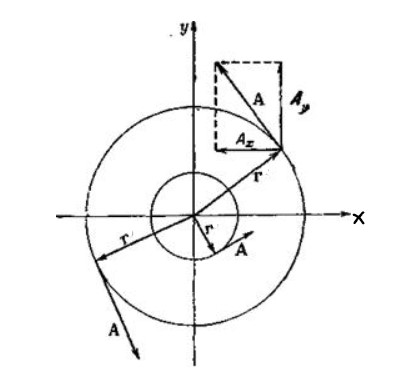
\includegraphics[width=1\linewidth]{pictures/30.1.jpg}
\caption{Однородное магнитное поле $\vec{B}$, направленное по оси $Oz$, соответствует векторному потенциалу $A_{\theta}= \frac{1}{2} rH$, который вращается вокруг этой оси. $r$ - расстояние до оси $Oz$.}
\end{wrapfigure}
\par Тогда можем взять $\vec{A} = \frac{1}{2}(-y, x, 0)H$. Поскольку x-компонента пропорциональна -y, а y-компонента пропорциональна x, то вектор  должен быть перпендикулярен вектору $\vec{r}$, проведенному от оси $Oz$. Кроме того, величина $\vec{A}$ пропорциональна $\sqrt{x^2+y^2}$ и, следовательно, пропорциональна $\vec{r}$. Поэтому для однородного поля можно записать $\vec{A}= \frac{1}{2} \vec{B} \times \vec{r}$ или же $A_{\theta}= \frac{1}{2} rH$ (\textbf{радиальная калибровка}). Векторный потенциал  вращается вокруг оси $Oz$, как показано на рисунке 30.1. Если, например, поле $\vec{B}$ есть поле внутри соленоида вдоль его оси, то векторный потенциал циркулирует точно таким же образом, как и токи в соленоиде.
\par Выберем калибровку $\vec{A} = (-y, 0, 0)H$.
\par \textbf{2. Распишем уравнение покомпонентно.}
$$\frac{\left(-i\hbar \frac{\partial}{\partial x} - \frac{e}{c}(-Hy) \right)^2}{2m}\psi - \frac{\hbar^2}{2m} \frac{\partial^2}{\partial y^2}\psi - \frac{\hbar^2}{2m} \frac{\partial^2}{\partial z^2}\psi =E \psi$$
\par Избавимся от производной по $z$: $\frac{(p_z)^2}{2m}$ - кинетическая энергия вдоль поля, частица не испытывает влияния, но в классике действует сила Лоренца и частица движется по окружности.
\par В уравнении нет в явном виде координат $x$ и $z$ - они циклические, значит, можем произвести разделение переменных, введя замену (а после опустить волну в уравнении):
$$ \psi = \widetilde{\psi} e^{i k_z z}e^{i k_x x} $$
$$\frac{1}{2m} \underbrace{\left(\hbar k_x + \frac{eH}{c} y \right)^2}_{U} \psi - \frac{\hbar^2}{2m} \frac{\partial^2 \psi}{\partial y^2} = \left(E - \frac{\hbar^2 k^2_z}{2m} \right) \psi$$
\par где $U$ - потенциал гармонического осциллятора со смещенной координатой $y$ на $const$.
$$\psi^{\prime \prime} + \frac{2m}{\hbar^2} \left(\left(E- \frac{p^2_z}{2m} \right) - \frac{m}{2} w^2_H (y-y_0)^2 \right) \psi = 0$$
\par Здесь $y_0 = -\frac{c p_x}{eH}$ - положение центра орбиты, $e=-|e|$ - заряд электрона, $w_H = \frac{|e|H}{mc}$ - циклотронная частота. Спектр осциллятора: 
$$E= \frac{p^2_z}{2m} +\hbar w_H (n+1/2)$$ 
\par Это \textbf{уровень Ландау}. В 1930 году эту задачу решил Ландау (хотя Фок сделал это раньше), он  вычислил измеримые величины (сказал, что диамагнетизм системы подвижных носителей зарядов связан с тем, что при помещении заряженных частиц в магнитном поле траектории свободного движения частиц искривляются и возникает добавочное магнитное поле, противоположное внешнему, т. е. у системы заряженных частиц появляется добавочный диамагнитный момент. Этот диамагнетизм заметно проявляется при низких температурах (ниже температуры вырождения) и может наблюдаться в вырожденном газе свободных электронов и у электронов проводимости в металлах, полуметаллах и полупроводниках). 
\par Решение полученного дифференциального уравнение дается спец-функциями - функциями Эрмита: $\psi = \Phi \left(\frac{y-y_0}{L_H} \right)$, где $L_H= \sqrt{\frac{\hbar c}{eH}}$ - магнитная длина.
\par //куча слов//
\par Тот факт, что энергия не зависит от $p_x$ ($k_x$) означает, что данные состояния вырождены, причем вырождение бесконечно-кратное. Куда делось движение по окружности при $\hbar \rightarrow 0 $ - исчезла калибровочная инвариантность.

\par //Наверное, надо еще включить все остальное про ток, связанный с квантовомеханическим электроном, и про вывод плотности потока вероятности...//

